\documentclass[a4paper,12pt]{article}
\usepackage{amssymb} % needed for math
\usepackage{amsmath} % needed for math
\usepackage[utf8]{inputenc} % this is needed for german umlauts
\usepackage[ngerman]{babel} % this is needed for german umlauts
\usepackage[T1]{fontenc}    % this is needed for correct output of umlauts in pdf
\usepackage[margin=2.5cm]{geometry} %layout
\usepackage{booktabs}
\usepackage{graphicx}
\usepackage{csquotes}
\usepackage[nonumberlist]{glossaries}
\usepackage{enumitem}
\usepackage[capposition=top]{floatrow}
\usepackage{verbatim}
\usepackage{indentfirst} % Adds indent for the first paragraph after a {/section}
\usepackage{url}
\newcommand\purl[1]{\protect\url{#1}}



\deftranslation[to=ngerman]{Glossary}{\section{Stichwortverzeichnis}}

\makeatletter
\newenvironment{mycode}
 {\def\@xobeysp{\ }\verbatim\rightskip=0pt plus 6em\relax}
 {\endverbatim}
\makeatother

\setitemize{align=parleft, labelsep=0.5cm}


\makenoidxglossaries



\title{Balanced Banana}
\author{Niklas Lorenz \and Thomas Häuselmann \and Rakan Zeid Al Masri \and Christopher Lukas Homberger \and Jonas Seiler}


%%%%%%%%%%%%%%%%%%%%%%%%%%%%%%%%%%%%%%%%%%%%%%%%%%%%%%%%%%%%%%%%%%%%%%
% Create a shorter version for tables. DO NOT CHANGE               	 %
%%%%%%%%%%%%%%%%%%%%%%%%%%%%%%%%%%%%%%%%%%%%%%%%%%%%%%%%%%%%%%%%%%%%%%
\newcommand\addrow[2]{#1 &#2\\ }

\newcommand\addheading[2]{#1 &#2\\ \hline}
\newcommand\tabularhead{\begin{tabular}{lp{13cm}}
\hline
	}

\newcommand\addmulrow[2]{ \begin{minipage}[t][][t]{2.5cm}#1\end{minipage}%
   &\begin{minipage}[t][][t]{8cm}
    \begin{enumerate} #2   \end{enumerate}
    \end{minipage}\\ }

\newenvironment{usecase}{\tabularhead}
{\hline\end{tabular}}

\usepackage{microtype}

\begin{document}
\pagenumbering{roman}
\begin{titlepage}
    \begin{center}
    
     \vspace*{0.8cm}
 
        
\includegraphics[width=0.5\textwidth]{balancedbanana}
        \vspace*{1cm}
 
        \Huge
        \textbf{Balanced Banana}
 
        \vspace{0.5cm}
        \LARGE
        A Distributed Task Scheduling System
        
        \vspace{0.5 cm}
        \LARGE
        Pflichtenheft
 
        \vspace{1.5cm}

        \large
        \textbf{Niklas Lorenz, Thomas Häuselmann, Rakan Zeid Al Masri, Christopher Lukas Homberger und Jonas Seiler}
 
        \vspace*{0.5cm}

        \textbf{\today}
 
       
        
 
    \end{center}
\end{titlepage}         % Deckblatt.tex laden und einfügen
\setcounter{page}{2}
\tableofcontents          % Inhaltsverzeichnis ausgeben
\clearpage
\pagenumbering{arabic}

% Document starts here.
\section{Einleitung}
\vspace{1cm}
Mit diesem Entwurfsdokument möchten wir die Architektur unseres Programms vorstellen und erläutern. Das Dokument zeigt zunächst die Konzeption unseres Systems auf hohem Niveau. Anschließend werden die Besonderheiten der einzelnen Module und die Klassen innerhalb der Module erläutert. Darüber hinaus sind Sequenzdiagramme verfügbar, um die Funktionalität unseres Programms weiter zu veranschaulichen und ein tieferes, praktischeres Verständnis der Funktionsweise zu vermitteln.
\clearpage
\section{Aufbau}

\subsection{Architektur}
% Hier soll die verschiedenen Teile unseres Programms erklärt werden.

Mit Rücksicht auf die verschiedenen Aspekte, die zur Verwendung unseres Programms gehören, wurde unser Programm in 3 Blöcke unterteilt. Diese 3 Blöcke arbeiten als jeweils eigenständiges Programm:\newline
Die Client Anwendung, die für die Interaktion mit einem menschlichen Benutzer zuständig ist.\newline
Die Server Anwendung, die den Hauptteil der Logik des Programms ausmacht. Sie ist für die Verteilung der Benutzeraufgaben auf die Arbeiter zuständig, was den Hauptaspekt unseres Programms darstellt.\newline
Die Worker Anwendung, die für die tatsächliche Ausführung der Benutzeraufgaben auf den verfügbaren Arbeiterrechnern zuständig ist.\newline
\newline
Zusätzlich existieren weitere Module, die in diesen Anwendungen Verwendung finden. So ist das Kommunikation-Modul dafür zuständig, dass sich die Anwendungen untereinander austauschen können und somit der Benutzer in der Lage ist, seine Aufgaben mithilfe der Client Anwendung in Auftrag zu geben und Abfragen zu seinen Aufgaben stellen kann.\newline
Ein weiteres Modul beschäftigt sich mit dem Einlesen von Befehlen auf der Befehlszeile. Dieses Modul findet Hauptsächlich in der Client Anwendung Verwendung, ist jedoch in allen 3 Anwendungen vorhanden, da diese gelegentlich auch mit der Befehlszeile interagieren müssen (mindestens einmal beim Anwendungsstart).
\newline
Das Modul Datenbank hingegen findet ausschließlich in der Server Anwendung Verwendung. Es dient dazu, die Informationen zur Ausführung des Verteilersystems zu sichern, und aus den vorhandenen Daten statistische Rückschlüsse zu ermöglichen, die einem Beobachter einen Überblick z.B. über die Auslastung der Arbeiter ermöglichen. Auch werden systemkritische Informationen hier gesichert, die einen Neustart des Systems oder Abbruch der Stromversorgung überleben müssen, um den korrekten Betrieb des Programms zu garantieren. Somit gehen Informationen bezüglich der in Auftrag gegebenen Aufgaben nicht verloren.
\newline
Das Modul Warteschlange realisiert eine Grundlage für die Verteilung von Benutzeraufgaben, die von den Benutzern gesetzte Prioritäten berücksichtigen soll. Die Warteschlange ermöglicht eine effiziente Auswahl der auszuführenden Aufgaben aus dem Pool aller Aufgaben.

\clearpage

\subsubsection{Datenbank}

	Die Datenbank enthält relevante Daten über verschiedene Entitäten in unserem Programm. Mit Hilfe von SQL-Queries kann unser Programm diese Daten abrufen und sinnvoll nutzen.  Unsere Datenbank verwendet ein relationales Datenbank-Managementsystem, um Informationen in verschiedenen Tabellen zu speichern. Darüber hinaus sind die Tabellen über Beziehungen miteinander verbunden, die den Sinn der Daten weiter verdeutlichen. Nachfolgend finden Sie ein Entity-Relationship-Diagramm, das zeigt, wie unsere Datenbank konzipiert ist:

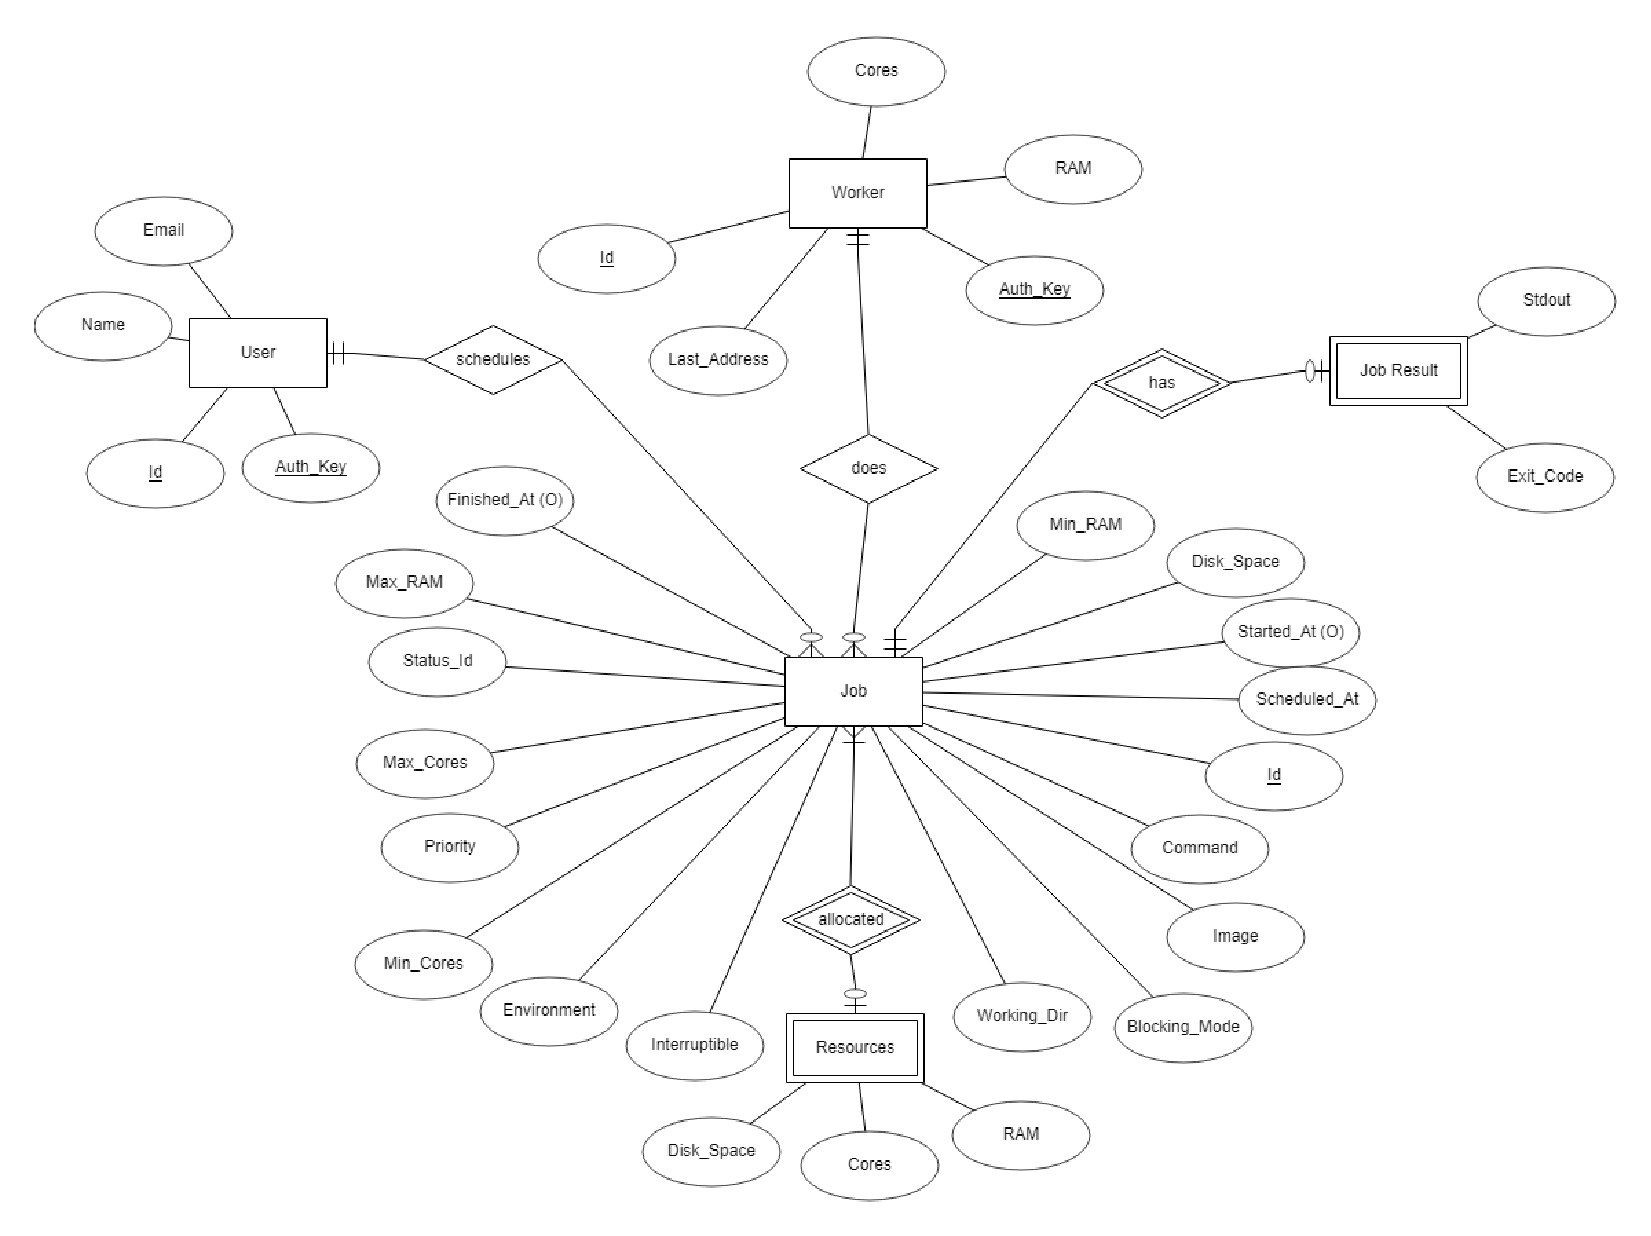
\includegraphics[width=\textwidth]{database_relational}

\clearpage
Die Datenbank ist in drei verschiedene Klassen unterteilt: Die Repository-, die Gateway- und die Factory-Klasse. Die Gateway-Klasse verwendet das Qt-Framework, um sich mit der Datenbank zu verbinden und die SQL-Queries durchzuführen. Die Factory-Klasse ist für die Erstellung von Objekten aus den vom Gateway zurückgegebenen Daten verantwortlich. Das Repository nutzt beide Klassen und dient als Schnittstelle für den Zugriff auf die Datenbank.\newline


\begin{figure}
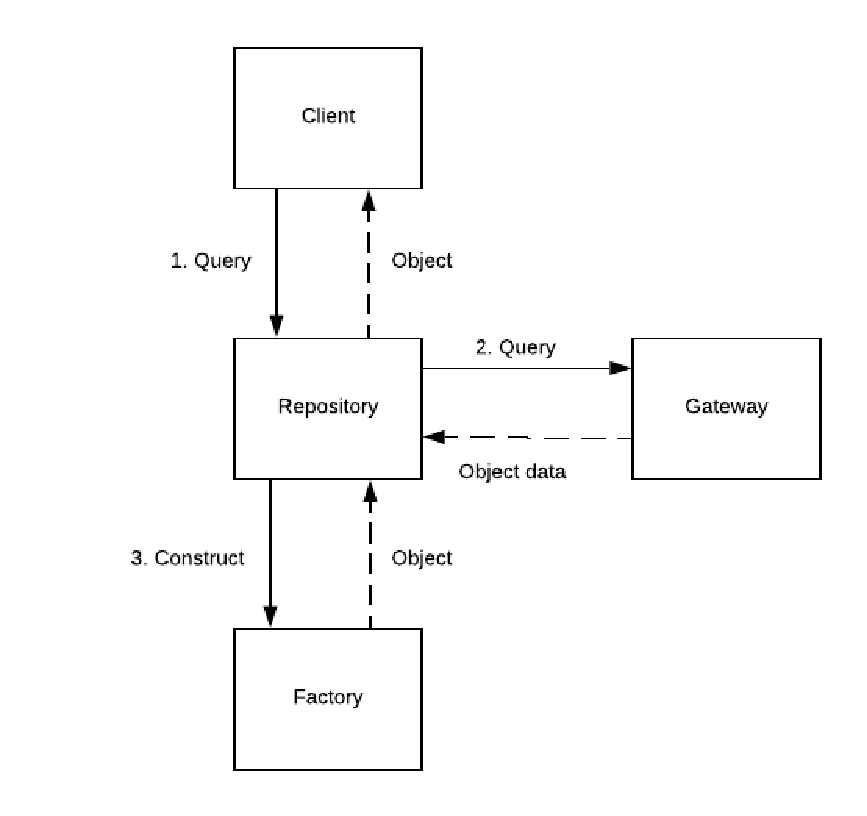
\includegraphics[width=\textwidth]{high_lvl_repository}
\floatfoot{High-Level-Darstellung des Datenbankdesigns}
\end{figure}

\clearpage
\subsection{Klassendiagramm}

% Übersicht aller Klassendiagramme




\clearpage
\section{Klassenbeschreibung}

\iffalse
Format:
\subsubsection{Klasse}

Kurze Beschreibung

\begin{itemize}[label={}]

	\item \textit{\textbf{Attribute}}
		\begin{itemize}[label={\textbullet}]
			\item \textit{name} beschreibung
		\end{itemize}

	\item \textit{\textbf{Methoden}}
		\begin{itemize}[label={\textbullet}]
			\item \textit{signatur} beschreibung
		\end{itemize}


\end{itemize}

\fi

\subsection{Datenbank}
\subsubsection{Model}
%Show the class diagram for it first

\subsubsection{Repository}

Die Repository-Klasse ist die Schnittstelle, die der Rest des Programms verwendet, um SQL-Queries durchzuführen und deren Ergebnisse zu interpretieren. Es verwendet die Gateway-Klasse, um die SQL-Queries durchzuführen und erzeugt ein Objekt, indem es der Factory-Klasse die von Gateway zurückgegebenen Daten gibt.

	\begin{itemize}[label={}]
	
		\item \textit{\textbf{Methoden}}
			\begin{itemize}[label={\textbullet}]
				\item \textit{public uint64\_t addWorker(int auth\_key, int space, int ram, int cores, std::string address)} Fügt einen Worker zur Datenbank hinzu und gibt seine ID zurück.
				
				\item \textit{public bool removeWorker(uint64\_t id)} Löscht einen Worker aus dem DB. Gibt true zurück, wenn die Operation erfolgreich war, ansonsten false.
				
				\item \textit{public Worker getWorker(uint64\_t worker\_id)} Gibt den Worker mit der angegebenen ID zurück.
				
				\item \textit{public std::vector<std::shared\_ptr<Worker>> getWorkers()} Gibt alle Workers zurück.
				
				\item \textit{public uint64\_t addJob(uint64\_t user\_id, JobConfig config, std::chrono::time\_point schedule\_time, std::string command)} Fügt einen Job zur Datenbank hinzu und gibt seine ID zurück. 
				
				\item \textit{public bool removeJob(uint64\_t job\_id)} Löscht einen Job aus dem DB. Gibt true zurück, wenn die Operation erfolgreich war, ansonsten false.
				
				\item \textit{public Job getJob(uint64\_t job\_id)} Gibt den Job mit der angegebenen ID zurück.
				
				\item \textit{public std::vector<std::shared\_ptr<Job>> getJobs()} Gibt alle Jobs zurück.
				
				\item \textit{public uint64\_t addUser(std::string name, std::string email, int auth\_key)} Fügt einen User zur Datenbank hinzu und gibt seine ID zurück. 
				
				\item \textit{public bool removeUser(uint64\_t user\_id)} Löscht einen User aus dem DB. Gibt true zurück, wenn die Operation erfolgreich war, ansonsten false.
				
				\item \textit{public User getUser(uint64\_t user\_id)} Gibt den User mit der angegebenen ID zurück.
				
				\item \textit{public std::vector<std::shared\_ptr<User>> getUsers()} Gibt alle Users zurück.
				
				\item \textit{public bool startJob(uint64\_t job\_id, uint64\_t worker\_id, specs specs, std::chrono::time\_point start\_time)} Aktualisiert den Eintrag eines Jobs in der Datenbank mit einer Startzeit, den zugewiesenen Ressourcen und dem zugeordneten Mitarbeiter. Gibt true zurück, wenn die Operation erfolgreich war, ansonsten false.
				
				\item \textit{public bool finishJob(uint64\_t job\_id, std::chrono::time\_point finish\_time, std::string stdout, int8\_t exit\_code)} Aktualisiert den Eintrag eines Jobs mit Endzeit, Ausgabe und Exitcode. Gibt true zurück, wenn die Operation erfolgreich war, ansonsten false.
				
				\item \textit{public job\_result getJobResult(uint64\_t job\_id)} Gibt die Ergebnisse eines \textbf{fertigen} Jobs zurück.
								
			\end{itemize}
			
	\end{itemize}
\subsubsection{Gateway}

Die Gateway-Klasse verbindet sich mit der Datenbank und führt die SQL-Queries aus.

\begin{itemize}[label={}]

	\item \textit{\textbf{Attribute}}
		\begin{itemize}[label={\textbullet}]
			\item \textit{QSqlDatabase db} Verwaltet die Verbindung zur Datenbank. 
		\end{itemize}

	\item \textit{\textbf{Methoden}}
		\begin{itemize}[label={\textbullet}]
			\item \textit{public uint64\_t addWorker(int auth\_key, int space, int ram, int cores, std::string address)} Fügt einen Worker zur Datenbank hinzu und gibt seine ID zurück.
				
				\item \textit{public bool removeWorker(int uint64\_t)} Löscht einen Worker aus dem DB. Gibt true zurück, wenn die Operation erfolgreich war, ansonsten false.
				
				\item \textit{public worker\_details getWorker(uint64\_t worker\_id)} Gibt die Daten des Workers mit der angegebenen ID zurück.
				
				\item \textit{public std::vector<std::shared\_ptr<worker\_details>> getWorkers()} Gibt die Daten jedes Mitarbeiters zurück.
				
				\item \textit{public uint64\_t addJob(uint64\_t user\_id, JobConfig config, std::chrono::time\_point schedule\_time, std::string command)} Fügt einen Job zur Datenbank hinzu und gibt seine ID zurück. 
				
				\item \textit{public bool removeJob(uint64\_t job\_id)} Löscht einen Job aus dem DB. Gibt true zurück, wenn die Operation erfolgreich war, ansonsten false.
				
				\item \textit{public job\_details getJob(uint64\_t job\_id)} Gibt die Daten des Jobs mit der angegebenen ID zurück.
				
				\item \textit{public std::vector<std::shared\_ptr<job\_details>> getJobs()} Gibt die Daten jedes Jobs zurück.
				
				\item \textit{public uint64\_t addUser(std::string name, std::string email, int auth\_key)} Fügt einen User zur Datenbank hinzu und gibt seine ID zurück. 
				
				\item \textit{public bool removeUser(uint64\_t user\_id)} Löscht einen User aus dem DB. Gibt true zurück, wenn die Operation erfolgreich war, ansonsten false.
				
				\item \textit{public user\_details getUser(uint64\_t user\_id)} Gibt die Daten des Users mit der angegebenen ID zurück
				
				\item \textit{public std::vector<std::shared\_ptr<user\_details>> getUsers()} Gibt die Daten jedes Users zurück.
				
				\item \textit{public bool startJob(uint64\_t job\_id, uint64\_t worker\_id, specs specs, std::chrono::time\_point start\_time)} Aktualisiert den Eintrag eines Jobs in der Datenbank mit einer Startzeit, den zugewiesenen Ressourcen und dem zugeordneten Mitarbeiter. Gibt true zurück, wenn die Operation erfolgreich war, ansonsten false.
				
				\item \textit{public bool finishJob(uint64\_t job\_id, std::chrono::time finish\_time, std::string stdout, int8\_t exit\_code)} Aktualisiert den Eintrag eines Jobs mit Endzeit, Ausgabe und Exitcode. Gibt true zurück, wenn die Operation erfolgreich war, ansonsten false.
				
				\item \textit{public job\_result getJobResult(uint64\_t job\_id)} Gibt die Ergebnisse eines \textbf{fertigen} Jobs zurück.
		\end{itemize}


\end{itemize}

\subsubsection{Factory}

Erzeugt Objekte aus gegebenen Daten.

\begin{itemize}[label={}]

	\item \textit{\textbf{Methoden}}
		\begin{itemize}[label={\textbullet}]
			\item \textit{public Job createJob(job\_details info)} Erzeugt ein Job-Objekt.
			
			\item \textit{public Worker createWorker(worker\_details info)} Erzeugt ein Worker-Objekt.
			
			\item \textit{public User createUser(user\_details info)} Erzeugt ein User-Objekt.
		\end{itemize}


\end{itemize}
\subsubsection{struct \purl{user_details}}

Eine struct, die alle relevanten Userdaten kapselt.

\begin{itemize}[label={}]

	\item \textit{\textbf{Attribute}}
		\begin{itemize}[label={\textbullet}]
			\item \textit{uint64\_t id} Eine eindeutige ID zur Identifizierung des Users.
			
			\item \textit{std::string name} Der Name des Users.
			
			\item \textit{std::string email} Die Email des Users.
			
			\item \textit{authkey} to be filled
		\end{itemize}


\end{itemize}

\subsubsection{struct specs}

Eine struct, die alle relevanten Hardware-Spezifikationen des Rechners kapselt.


\begin{itemize}[label={}]

	\item \textit{\textbf{Attribute}}
		\begin{itemize}[label={\textbullet}]
			\item \textit{int space} Speicherplatz.
			
			\item \textit{int ram} Random-Access Memory.
			
			\item \textit{int cores} Anzahl der CPU-Kerne.
			
		\end{itemize}


\end{itemize}
\subsubsection{struct \purl{worker_details}}

Eine struct, die alle relevanten Workerdaten kapselt.


\begin{itemize}[label={}]

	\item \textit{\textbf{Attribute}}
		\begin{itemize}[label={\textbullet}]
			\item \textit{uint64\_t id} Eine eindeutige ID zur Identifizierung des Workers.
			
			\item \textit{specs specs} Hardware-Spezifikationen des Rechners.
			
			\item \textit{std::string address}
			
			\item \textit{authkey} to be filled
		\end{itemize}


\end{itemize}
\clearpage

\subsubsection{struct \purl{job_details}}

Eine struct, die alle relevanten Jobdaten kapselt.

\begin{itemize}[label={}]

	\item \textit{\textbf{Attribute}}
		\begin{itemize}[label={\textbullet}]
			\item \textit{JobConfig config} Enthält die Konfiguration eines Jobs.
			
			\item \textit{uint64\_t user\_id} Die ID des Users, der diesen Job gescheduled hat.
			
			\item \textit{int status} Der Statuscode eines Jobs.
			
			\item \textit{uint64\_t id} Eine eindeutige ID zur Identifizierung des Jobs.
			
			\item \textit{std::string command} Der Befehl des Jobs, der in der Befehlszeile eingegeben wurde.
			
			\item \textit{std::chrono::time\_point schedule\_time} Die Uhrzeit, zu der der Job gescheduled wurde.
			
			\item \textit{std::chrono::time\_point start\_time} Die Uhrzeit, zu der der Job gestartet wurde.
			
			\item \textit{std::chrono::time\_point finish\_time} Die Uhrzeit, zu der der Job beendet wurde.
			
			\item \textit{specs allocated\_specs} Die Hardware-Ressourcen, die dem Job zugewiesen wurden.

		\end{itemize}


\end{itemize}
\clearpage

\subsection{Configfiles}

\subsubsection{enum Priority}

Eine Aufzählung aller möglichen Prioritäten, die ein Job haben kann.
\begin{itemize}[label={}]
	\item \textit{\textbf{Items}}
		\begin{itemize}[label={\textbullet}]
			\item \textit{low} Priorität für Jobs, deren zeitnahe Abarbeitung unwichtig ist.
			\item \textit{normal} Priorität für Jobs, die zeitnahe abgearbeitet werden sollen.
			\item \textit{high} Priorität für Jobs, die sehr schnell abgearbeitet werden müssen.
			\item \textit{emergency} Priorität für Jobs, die umgehend bearbeitet werden müssen. Der Scheduler kann eventuell sogar andere Jobs zeitweise unterbrechen um andere Jobs mit dieser Priorität zu bearbeiten.
		\end{itemize}
\end{itemize}

\subsubsection{JobConfig}

Eine Sammlung an allen möglichen Einstellungen, die beschreiben, wie ein Job bearbeitet, bzw. eingeplant werden soll.

\begin{itemize}[label={}]

	\item \textit{\textbf{Attribute}}
		\begin{itemize}[label={\textbullet}]
			\item \textit{std::optional<uint32\_t> min\_ram\_} Minimal benötigter Hauptspeicher
			\item \textit{std::optional<uint32\_t> max\_ram\_} Maximal benötigter Hauptspeicher
			\item \textit{std::optional<uint32\_t> min\_cpu\_count\_} Minimal benötigte CPU Kerne
			\item \textit{std::optional<uint32\_t> max\_cpu\_count\_} Maximal zu verwendende CPU Kerne
			\item \textit{std::optional<bool> blocking\_mode\_} Ob der Client auf den Abschluss der Aufgabe wartet
			\item \textit{std::string email\_} Zu benachrichtigende Adresse
			\item \textit{std::optional<Priority> priority\_} Priorität des Jobs in der Warteschlange
			\item \textit{std::string image\_} Zu verwendendes Docker Image
			\item \textit{std::optional<std::vector<std::string>> environment\_} Liste an Umgebungsvariablen
			\item \textit{std::optional<bool> interruptible\_} Ob der Job unterbrechbar ist.
			\item \textit{std::optional<std::filesystem::path> current\_working\_dir\_} Verzeichnis, von dem aus der Job im Container ausgeführt werden soll.
		\end{itemize}

	\item \textit{\textbf{Methoden}}
		\begin{itemize}[label={\textbullet}]
			\item \textit{JobConfig()} Erstellt eine leere JobConfig
			\item \textit{JobConfig(std::stringstream \&)} Deserialisiert eine JobConfig aus dem übergebenen Stream
			\item \textit{JobConfig(std::filesystem::path \&)} Lädt eine serialisierte JobConfig aus dem Dateisystem an dem angegebenen Pfad.
			\item \textit{void set\_min\_ram(std::optional<uint32\_t>)} Setter für min\_ram\_
			\item \textit{void set\_max\_ram(std::optional<uint32\_t>)} Setter für max\_ram\_
			\item \textit{void set\_min\_cpu\_count(std::optional<uint32\_t>)} Setter für min\_cpu\_count\_
			\item \textit{void set\_max\_cpu\_count(std::optional<uint32\_t>)} Setter für max\_cpu\_count\_
			\item \textit{void set\_blocking\_mode(std::optional<bool>)} Setter für blocking\_mode\_
			\item \textit{void set\_email(std::string \&)} Setter für email\_
			\item \textit{void set\_priority(std::optional<Priority>)} Setter für priority\_
			\item \textit{void set\_image(std::string \&)} Setter für image\_
			\item \textit{void set\_environment(std::optional<std::vector<std::string>> \&)} Setter für environment\_
			\item \textit{void set\_interruptible(std::optional<bool>)} Setter für interruptible\_
			\item \textit{void set\_current\_working\_dir(std::optional<std::filesystem::path> \&)} Setter für
			current\_working\_dir\_
			\item \textit{std\_optional<uint32\_t> min\_ram()} Getter für min\_ram\_
			\item \textit{std\_optional<uint32\_t> max\_ram()} Getter für max\_ram\_
			\item \textit{std\_optional<uint32\_t> min\_cpu\_count()} Getter für min\_cpu\_count\_
			\item \textit{std\_optional<uint32\_t> max\_cpu\_count()} Getter für max\_cpu\_count\_
			\item \textit{std\_optional<bool> blocking\_mode()} Getter für blocking\_mode\_
			\item \textit{std::string \&email()} Getter für email\_
			\item \textit{std\_optional<Priority> priority()} Getter für priority\_
			\item \textit{std::string \&image()} Getter für image\_
			\item \textit{std\_optional<std::vector<std::string>> \&environment()} Getter für environment\_
			\item \textit{std\_optional<bool> interruptible()} Getter für interruptible\_
			\item \textit{std\_optional<std::filesystem::path> \&current\_working\_dir()} Getter für current\_working\_dir\_
			\item \textit{void Serialize(std::stringstream \&)} Schiebt die serialisierte JobConfig in den angegebenen Stream.
			\item \textit{void Save(std::filesystem::path \&)} Speichert die JobConfig im Filesystem an der angegebenen Stelle. 
			\item \textit{void Merge(JobConfig \&)} Füllt diese JobConfig mit Werten aus der übergebenen JobConfig auf. In beiden Configs vorhandene Werte werden nicht überschrieben.
		\end{itemize}


\end{itemize}
\clearpage
\subsubsection{SchedulerConfig}

Wrapper für eine Hashmap, der auch eine Möglichkeit zum Speichern und Laden ins Filesystem bietet und als Speicher für verschiedene Regeln beim Einplanen der Jobs dient.

\begin{itemize}[label={}]

	\item \textit{\textbf{Attribute}}
		\begin{itemize}[label={\textbullet}]
			\item \textit{std::map<std::string, std::string> values\_} Hashmap, die alle Regeln enthält.
		\end{itemize}

	\item \textit{\textbf{Methoden}}
		\begin{itemize}[label={\textbullet}]
			\item \textit{SchedulerConfig()} Erzeugt eine leere SchedulerConfig
			\item \textit{SchedulerConfig(std::filesystem::path \&)} Lädt eine serialisierte SchedulerConfig aus dem Filesystem
			\item \textit{size\_t count()} Gibt an wie viele Elemente sich in der Config befinden.
			\item \textit{Get(std::string \&)} Gibt das Element zurück, das der übergebenen Regel zugeordnet wurde.
			\item \textit{Set(std::string \&key, std::string \&value)} Setzt den Wert der Regel mit dem übergebenen key auf den übergebenen Wert.
			\item \textit{Save(std::filesystem::path \&)} Schreibt die Config in das Filesystem an die angegebene Stelle.
			\item \textit{Contains(std::string \&)} Gibt an, ob sich in der Config eine Regel mit dem angegebenen key befindet.
		\end{itemize}


\end{itemize}
\clearpage
\subsection{Client}

\subsubsection{Model}

% Diagramm

\subsubsection{CommandLineProcessor}

Der Command Line Processor (CLP) ist dafür zuständig, die Benutzereingabe auf der Befehlszeile in eine für das Programm verwendbare Struktur zu überführen. Es werden die Argumente auf der Befehlszeile eingelesen und mit vom Benutzer in einer Konfigurationsdatei angegebenen Standardwerten ergänzt. Anhand der Angaben auf der Befehlszeile kann erkannt werden, um welchen Typ von Befehl es sich handelt, und welche Parameter für die Ausführung des Befehls vorhanden sein müssen.

\begin{itemize}[label={}]

	\item \textit{\textbf{Methoden}}
		\begin{itemize}[label={\textbullet}]
			\item \textit{public Task process(char** argv, int* argc)} Verarbeitet Argumente der Befehlszeile. Weist jedem Argument zuerst den auf der Befehlszeile spezifizierten Wert, dann den vom Benutzer in einer Konfigurationsdatei hinterlegten Wert zu. Argumente, die nicht auf der Befehlszeile oder in der Konfigurationsdatei vorhanden sind, werden von dem Server mit Standardwerten verfollständigt.\newline
			\newline
			argv: Array der Bezeichner sowie Werte der Argumente\newline
			argc: Anzahl der Einträge in argv


			\item \textit{private void preProcess(char** argv, int* argc, std::shared\_ptr<Task> task)}
			Baut aus den übergebenen Argumenten einen Task auf.\newline
			Bestimmt den Typ der Anfrage (neue Aufgabe oder vorhandene Bearbeiten)\newline
			Hierbei werden komplexe Argumente von den eigentlichen Argumenten getrennt (z.B. wird der Aufgaben 	Startbefehl von den Argumenten unseres Programms abgetrennt, damit dies nicht zu Problemen in späteren
			Verarbeitungsschritten führt).\newline
			argv und argc werden dementsprechend angepasst.\newline
			\newline
			argv: Array der Bezeichner und Werte der Argumente\newline
			argc: Anzahl der Einträge in argv\newline
			task: Bekommt einen Aufgaben-Typ zugewiesen


			\item \textit{private void processArguments(char** argv, int* argc, std::shared\_ptr<Task> task)}
			Wertet die Argumente der Befehlszeile aus und speichert sie in task.\newline
			Zusätzlich werden die Argumente aus der lokalen Konfigurationsdatei übernommen.\newline
			\newline
			argv: Array der Bezeichner und Werte der Argumente\newline
			argc: Anzahl der Einträge in argv\newline
			task: Enthält nach Abarbeitungsende alle auf der Befehlszeile eingelesenen Argumente sowie alle Standardargumente der lokalen Konfigurationsdatei


		\end{itemize}


\end{itemize}

\clearpage

\subsubsection{Task}

Ein Task ist eine Repräsentation eines auf der Befehlszeile eingegebenen Befehls. Er enthält Informationen, die für die Ausführung des gewünschten Befehls wichtig sind. Dazu gehören im wesentlichen Befehlstyp sowie Argumente.

\begin{itemize}[label={}]

	\item \textit{\textbf{Attribute}}
		\begin{itemize}[label={\textbullet}]
			\item \textit{taskCommand} Startbefehl für die eingereichte Aufgabe
			\item \textit{config} Konfiguration dieses Befehls. Argumente der Befehlszeile und der lokalen Konfigurationsdatei.
			\item \textit{type} Gibt an, um was für eine Form von Anfrage es sich handelt (Starte neue Aufgabe oder frage etwas über eine existierende Aufgabe ab)
		\end{itemize}

	\item \textit{\textbf{Methoden}}
		\begin{itemize}[label={\textbullet}]

			\item \textit{public int getType()} Gibt den Befehlstyp type zurück.

			\item \textit{public void setType(int type)} Setzt den Befehlstyp zu dem Angegebenen Typ. 

			\item \textit{public JobConfig getConfig()} Gibt Zugang zur Konfiguration des Befehls. Die Konfiguration kann von außerhalb beliebig modifiziert werden. 

			\item \textit{public std::string getTaskCommand()} Gibt den vom Benutzer spezifizierten Startbefehl der eingereichten Aufgabe (falls eine eingereicht wurde) so, wie er auf der Befehlszeile ausgeführt werden soll.

			\item \textit{public void setTaskCommand(const std::string\& taskCommand} Setzt den Startbefehl der eingereichten Aufgabe (falls eine eingereicht wurde).
		\end{itemize}

\end{itemize}

\subsubsection{Client}

Die Hauptklasse der Client Anwendung. Verarbeitet die Befehls des Benutzers und leitet diese weiter an den Server. Bei Bedarf kann auf eine Rückmeldung des Servers gewartet werden, die dem Benutzer auf der Befehlszeile angezeigt wird.

\begin{itemize}[label={}]

	\item \textit{\textbf{Methoden}}
		\begin{itemize}[label={\textbullet}]

			\item \textit{int main(char** argv, int* argc)} Wandelt den Befehl des Benutzers mithilfe des CommandLineProcessor in verwendbare Struktur um. Leitet diesen dann an den Server weiter. Bei Bedarf wird die Netzwerkkommunikation offen gehalten, bis der Server eine Rückmeldung gesendet hat. Nach Ausgabe der Rückmeldung ist der Befehl beendet und die Client Anwendung wird beendet.
			
		\end{itemize}

\end{itemize}

\clearpage


\subsection{Communication}

\subsubsection{Model}

% Diagramm


\subsubsection{AuthHandler}

Beschreibt Methoden zur Ausführung von Authentifizierungsversuchen auf dem Scheduler. Kann mithilfe verschiedener Protokolle eine Person authentifizieren. Dient der Sicherheit vor Verwechselung und Täuschung.

	\begin{itemize}[label={}]

	\item\textit{\textbf{Methoden}}
		\begin{itemize}[label={\textbullet}]
			\item\textit{public AuthHandler GetDefault(Communicator comm)} Gibt einen Allzweck AuthHandler zurück, der in jeder Situation funktioniert.
			\item\textit{public AuthHandler(Communicator comm)} Kontruktor des abstrakten AuthHandler kann nur von Unterklassen aufgerufen werden.
			\item\textit{public virtual void authenticate(std::shared\_ptr<User>, std::string password)} Authentifiziere einen Benutzer mithilfe eines Passworts.
			\item\textit{public void authenticate(std::shared\_ptr<User>, std::string signature)} Authentifiziere einen Benutzer mithilfe einer Signatur (nicht notwendigerweise ein Passwort)
			
		\end{itemize}

\end{itemize}


\subsubsection{SSHAuthHandler}

Implementiert einen AuthHandler, der mit dem localen OpenSSH client arbeitet.

	\begin{itemize}[label={}]

	\item\textit{\textbf{Methoden}}
		\begin{itemize}[label={\textbullet}]
			\item\textit{public void authenticate(std::string username, std::string password)} Implementiert die SSH Authentifizierung eines Benutzers mithilfe eines Passworts.
		\end{itemize}

\end{itemize}


\subsubsection{LDAPAuthHandler}

Implementiert einen AuthHandler, der mit der OpenLDAP C Api arbeitet.

	\begin{itemize}[label={}]

	\item\textit{\textbf{Methoden}}
		\begin{itemize}[label={\textbullet}]
			\item\textit{public void authenticate(std::string username, std::string password)} Implementiert die LDAP Authentifizierung eines Benutzers mithilfe eines Passworts.
		\end{itemize}

\end{itemize}


\subsubsection{ClientAuthMessage}

Nachricht für die Authentifizierung eines Clienten (Anwendung). Wird beim ersten Verbindungsaufbau verwendet. Bei weiteren Verbindungen können andere Nachrichten Typen erforderlich sein.

	\begin{itemize}[label={}]

	\item\textit{\textbf{Attribute}}
		\begin{itemize}[label={\textbullet}]
			\item\textit{std::string username} Der Name des zu authentifizierenden Benutzers.
			\item\textit{std::string password} Klartext des vom Benutzer angegebenen Passworts.
			\item\textit{std::string publickey} Ein öffentlicher Schlüssel, der im Authentifizierungsverfahren Anwendung findet. Wird vom Client bzw. Worker erzeugt.
		\end{itemize}

	\item\textit{\textbf{Methoden}}
		\begin{itemize}[label={\textbullet}]
			\item\textit{public ClientAuthMessage(std::string username, std::string password, std::string pubkey)}
			\item\textit{public void process(std::shared\_ptr<MessageProcessor> mp)}
		\end{itemize}

\end{itemize}


\subsubsection{PublicKeyAuthMessage}

Nachricht für die Authentifizierung eines Benutzers mittels eine public Key Verfahrens.

	\begin{itemize}[label={}]

	\item\textit{\textbf{Attribute}}
		\begin{itemize}[label={\textbullet}]
			
			\item\textit{std::string username} Der Name des zu authentifizierenden Benutzers.
			\item\textit{std::string usernamesignature} Eine Signatur, die dem Benutzer zugewiesen wurde.
		\end{itemize}

	\item\textit{\textbf{Methoden}}
		\begin{itemize}[label={\textbullet}]
			\item\textit{public void process(std::shared\_ptr<MessageProcessor> mp)}
			\item\textit{public PublicKeyAuthMessage(std::string username, std::string usernamesignature)}
		\end{itemize}

\end{itemize}


\subsubsection{AuthResult}

Ergebnis der Authentifizierung. Gibt im wesentlichen den Erfolg der Authentifizierung an.

	\begin{itemize}[label={}]

	\item\textit{\textbf{Attribute}}
		\begin{itemize}[label={\textbullet}]
			\item\textit{unsigned long status} Gibt an, wie die Authentifizierung ausgegangen ist. (Erfolg/Misserfolg)
		\end{itemize}

	\item\textit{\textbf{Methoden}}
		\begin{itemize}[label={\textbullet}]
			\item\textit{public unsigned long getStatus()}
		\end{itemize}

\end{itemize}


\subsubsection{WorkerAuthMessage}

Nachricht, die zur Authentifizierung eines Arbeiters dient. Hier wird im Allgemeinen kein komplexes Sicherheitsverfahren verwendet.

	\begin{itemize}[label={}]

	\item\textit{\textbf{Attribute}}
		\begin{itemize}[label={\textbullet}]
			\item\textit{std::string workername} Name des Arbeiters, der authentifiziert wird.
			\item\textit{std::string publickey} Ein public Key der in gleichnamigen Verfahren Anwendung findet.
		\end{itemize}

	\item\textit{\textbf{Methoden}}
		\begin{itemize}[label={\textbullet}]
			\item\textit{public void process(std::shared\_ptr<MEssageProcessor> mp)}
			\item\textit{public WorkerAuthMessage(std::string workername, std::string pubkey)}
		\end{itemize}

\end{itemize}


\subsubsection{Communicator}

Haupteinheit zur Kommunikation der verschiedenen Anwendungen. Ermöglicht senden und empfangen von Nachrichten, die von und zu anderen Einheiten des Systems gesendet werden. Verbirgt die Details der Netzwerkkommunikation vor anderen Teilen der Programme. Wird identisch in allen Anwendungen verwendet.

	\begin{itemize}[label={}]

	\item\textit{\textbf{Methoden}}
		\begin{itemize}[label={\textbullet}]
			\item\textit{public void listen(std::function<void(std::shared\_ptr<Message>)> callback)} Warte auf eine eingehende Nachricht. Ruft dann callback auf, mit der eingegangenen Nachricht als Parameter.
			\item\textit{public void send(Message message)} Sendet eine Nachricht an einen eindeutigen Empfänger.

		\end{itemize}

\end{itemize}


\subsubsection{SSLSocket}

Basis der verschlüsselten Kommunikation. Stellt Funktionalität zur sicheren Netzwerkkommunikation mithilfe des SSH Protokolls bereit.

	\begin{itemize}[label={}]

	\item\textit{\textbf{Methoden}}
		\begin{itemize}[label={\textbullet}]
			\item\textit{public void connect(std::string address} Verbindet sich mit einem Socket an der angegebenen Netzwerkadresse.
			\item\textit{public void listen(unsigned short port, std::function<void(std::shared\_ptr<SSLSocket>)> callback)} Wartet auf eine eingehende Nachricht an einem bestimmten Port. Ruft dann eine callback Methode auf mit dem relevanten Socket als Parameter. Die Callback Routine kann dann die Nachricht verarbeiten.
			\item\textit{public void send(const char* msg)} Sendet eine Nachricht an einen zuvor spezifizierten Empfänger.
			\item\textit{public void receive(char* data), size\_t size)} Nehme eine Netzwerknachricht entgegen, die in Form eines byte Streams am Netzwerkadapter ankam.
			\item\textit{public void listen(unsigned short port, std::function<void()> callback)} Wartet auf eine eingehende Nachricht und ruft dann eine callback methode auf, die dieses Ereigniss verarbeitet.

		\end{itemize}

\end{itemize}


\subsubsection{MessageProcessor}

Haupteinheit für die Verarbeitung eingegangener Nachrichten. Ein Message Processor kann den Typ einer Nachricht identifizieren und je nach Nachrichtentyp die benötigten Prozesse anstoßen, um die Nachricht zu verarbeiten.

	\begin{itemize}[label={}]

	\item\textit{\textbf{Methoden}}
		\begin{itemize}[label={\textbullet}]
			\item\textit{public void process(std::shared\_ptr<Message> msg)} Verarbeitet eine engegangene Nachricht, indem deren Typ identifiziert wird und mit den enthaltenen Daten Ereignisse angestoßen werden.
			\item\textit{private void handleInvalidMessage(std::shared\_ptr<Message> msg)} Sollte eine ungültige Nachricht eingegangen sein, wird diese an dieser Stelle behandelt. Kann von der konreten Implementierung des Message Processors abhängig sein.

		\end{itemize}

\end{itemize}


\subsubsection{ClientMP}

Message Processor für den Client. Hiermit verarbeitet die Client (Benutzer) Anwendung Nachrichten vom Server, wie zum Beispiel Rückmeldungen auf Statusabfragen.

	\begin{itemize}[label={}]

	\item\textit{\textbf{Methoden}}
		\begin{itemize}[label={\textbullet}]
			\item\textit{public void process(std::shared\_ptr<Message> msg)}

		\end{itemize}

\end{itemize}


\subsubsection{SchedulerClientMP}

Message Processor für den Server (Scheduler) der Nachrichten verarbeitet, die von Seiten einer Client (Benutzer) Anwendung kommen.

	\begin{itemize}[label={}]

	\item\textit{\textbf{Methoden}}
		\begin{itemize}[label={\textbullet}]
			\item\textit{public void process(std::shared\_ptr<Message> msg)}

		\end{itemize}

\end{itemize}


\subsubsection{SchedulerWorkerMP}

Message Processor für den Server (Scheduler) der Nachrichten verarbeitet, die von Seiten einer Worker Anwendung kommen.

	\begin{itemize}[label={}]

	\item\textit{\textbf{Methoden}}
		\begin{itemize}[label={\textbullet}]
			\item\textit{public void process(std::shared\_ptr<Message> msg)}

		\end{itemize}

\end{itemize}


\subsubsection{WorkerMP}

Message Processor für den Worker der Nachrichten verarbeitet, die von Seiten einer Server (Scheduler) Anwendung kommen.

	\begin{itemize}[label={}]

	\item\textit{\textbf{Methoden}}
		\begin{itemize}[label={\textbullet}]
			\item\textit{public void process(std::shared\_ptr<Message> msg)}

		\end{itemize}

\end{itemize}


\subsubsection{Message}

Basis jeder Nachricht, die von den Anwendungen aneinander versendet werden können. Erzwingt die Möglichkeit zur Eindeutigen Identifikation einer Nachricht anhand einer Id sowie die Möglichkeit eine Nachricht Netzwerkfähig zu machen und aus einer Netzwerknachricht zu rekonstruieren.

	\begin{itemize}[label={}]

	\item\textit{\textbf{Attribute}}
		\begin{itemize}[label={\textbullet}]
			\item\textit{protected const unsigned int typeId} Eindeutige Nummer, die eine Nachricht identifiziert. Wird verwendet um verschiedene Nachrichtentypen mit unterschiedlichen Daten zu unterscheiden.
			
		\end{itemize}

	\item\textit{\textbf{Methoden}}
		\begin{itemize}[label={\textbullet}]
			\item\textit{public void process(std::shared\_ptr<MessageProcessor> mp)} Verarbeite diese Nachricht mithilfe des angegebenen Message Processors.
			\item\textit{public std::string serialize()} Wandle die Nachricht in eine Abfolge von bytes um, die über das Netzwerk versendet werden kann.
			\item\textit{public std::shared\_ptr<Message> deserialize(const char* msg, unsigned int size)} Rekonstruieren die Nachricht aus einer folge von bytes, die über das Netzwerk angekommen sind.

		\end{itemize}

\end{itemize}


\subsubsection{SnapshotMessage}

Nachricht, die das Erstellen eines Snapshots einer laufenden Aufgabe auf einem Worker anfordert. Wird vom Scheduler an einen Worker versendet.

	\begin{itemize}[label={}]

	\item\textit{\textbf{Attribute}}
		\begin{itemize}[label={\textbullet}]
			\item\textit{unsigned long jobid} Welche Aufgabe soll gesichert werden?
			\item\textit{bool stop} Soll während dem Erstellen des Snapshots die Ausführung der Aufgabe pausiert werden?
			
		\end{itemize}

	\item\textit{\textbf{Methoden}}
		\begin{itemize}[label={\textbullet}]
			\item\textit{public void process(std::shared\_ptr<MessageProcessor>)}
			\item\textit{public SnapshotMessage(unsigned long jobid, bool stop)}

		\end{itemize}

\end{itemize}


\subsubsection{RegistrationMessage}

Nachricht, um sich bei einer anderen Anwendung anzumelden. Wird primär zwischen Server und Worker verwendet, damit die Worker wissen wie sie einen Scheduler ansprechen können und der Scheduler alle verfügbaren Worker kennen kann.

	\begin{itemize}[label={}]

	\item\textit{\textbf{Methoden}}
		\begin{itemize}[label={\textbullet}]
			\item\textit{public void process(std::shared\_ptr<MessageProcessor>)}

		\end{itemize}

\end{itemize}


\subsubsection{HardwareDetailMessage}

Nachricht, die Informationen über die Hardware eines Workers enthält. Wird vom Worker zum Scheduler gesendet.

	\begin{itemize}[label={}]

	\item\textit{\textbf{Attribute}}
		\begin{itemize}[label={\textbullet}]
			\item\textit{int coreCount} Wie viele CPU Kerne können für eine Aufgabe verwendet werden.
			\item\textit{int ramSize} Wie viel Arbeitsspeicher ist auf dem Worker vorhanden.
			\item\textit{std::string osIdentifier} Welches Betriebssystem verwendet der Worker.
			
		\end{itemize}

	\item\textit{\textbf{Methoden}}
		\begin{itemize}[label={\textbullet}]
			\item\textit{public void process(std::shared\_ptr<MessageProcessor>)}
			\item\textit{public HardwareDetailMessage(int coreCount, int ramSize, std::string osIdentifier)}

		\end{itemize}

\end{itemize}


\subsubsection{TaskMessage}

Nachricht, die Informationen zu einer Aufgabe übermittelt. Wird von Client zu Server gesendet.

	\begin{itemize}[label={}]

	\item\textit{\textbf{Attribute}}
		\begin{itemize}[label={\textbullet}]
			\item\textit{Task task} Objekt, welches Informationen über den vom Benutzer angeforderten Befehl enthält. Siehe Task.
			
		\end{itemize}

	\item\textit{\textbf{Methoden}}
		\begin{itemize}[label={\textbullet}]
			\item\textit{public void process(std::shared\_ptr<MessageProcessor>)}
			\item\textit{public TaskMessage(Task task)}

		\end{itemize}
\end{itemize}
\subsection{Scheduler}

\subsubsection{Queue}

Die Oberklasse einer Warteschlangen-Implementierung. Hier werden alle nötigen Methoden für eine spezielle Implementierung einer Warteschlange definiert, sowie Default-Rückgabewerte falls diese nicht implementiert wurden. Eine spezielle Warteschlange soll als konkrete Strategie diese Klasse erweitern.

\begin{itemize}[label={}]

\item \textit{\textbf{Methoden}}
\begin{itemize}[label={\textbullet}]
	
	\item \textit{void addTask(Job job)} Fügt der Warteschlange ein Job hinzu. Standardmäßig werden hier Jobs nur mit angefragter ID entfernt.

\item \textit{int getPos(int id)} Gibt die Position des Tasks mit der übergebenen ID aus. Standardmäßig wird hier "-1" ausgegeben.

\item \textit{Job getJob(int id)} Gibt den Job mit der angegeben ID aus der Warteschlange heraus. Dies ist eine Fallback-Methode und sollte in allen Warteschlangen-Strategien ersetzt werden. 

\item \textit{void update()} Wird regelmäßig vom Scheduler aufgerufen. Standardmäßig passiert nichts. Diese Methode soll von einer konkreten Strategie für regelmäßige Checks benutzt werden.

\end{itemize}

\end{itemize}

\subsubsection{PriorityQueue}

Eine spezielle Implementierung einer Warteschlange. Sortiert Tasks nach Prioritäten.

\begin{itemize}[label={}]

\item \textit{\textbf{Methoden}}
\begin{itemize}[label={\textbullet}]

\item \textit{void addTask(Job job)} Fügt der Warteschlange ein Job hinzu. Dieser wird entsprechend seiner Priorität weiter vorne eingestuft je wichtiger.

\item \textit{int getPos(int id)} Gibt die Position des Tasks mit der übergebenen ID aus.

\item \textit{Job getJob(int Ram, int Cores)} Gibt den wichtigsten Job, also den mit der höchsten Priorität,  aus, der zu den übergebenen Spezifikationen passt.

\item \textit{void update()} Überprüft ob ein Job bereits 24 Stunden in der Warteschlange verbracht hat und erhöht gegebenenfalls seine Priorität.

\end{itemize}

\end{itemize}

\clearpage

\subsubsection{Scheduler}

Die Hauptklasse des Schedulers. Hierdurch werden Befehle und Datenbankzugriffe gesteuert.
\begin{itemize}[label={}]
	
	\item \textit{\textbf{Methoden}}
	\begin{itemize}[label={\textbullet}]
		
		\item \textit{void onTaskMessage(Message message)} Verarbeitet den erhaltenen Befehl entsprechend und führt den Inhalt aus.
		
		\item \textit{void update()} Prüft alle Worker nach Verbindung und Status und updated gegebenfalls andere Module
		
		\item \textit{void intialize()} Stellt Verbindungen zu Workern her und versucht einen Status aus der Datenbank herzustellen. 
		
	\end{itemize}
	
\end{itemize}



\clearpage

\section{Abläufe}
\subsection{Repository Pattern Beispielverwendung}

Das folgende Sequenzdiagramm veranschaulicht, wie die \textit{getWorker(uint64\_t worker\_id)} funktioniert und, was noch wichtiger ist, wie das Repository-Pattern als Ganzes funktioniert.

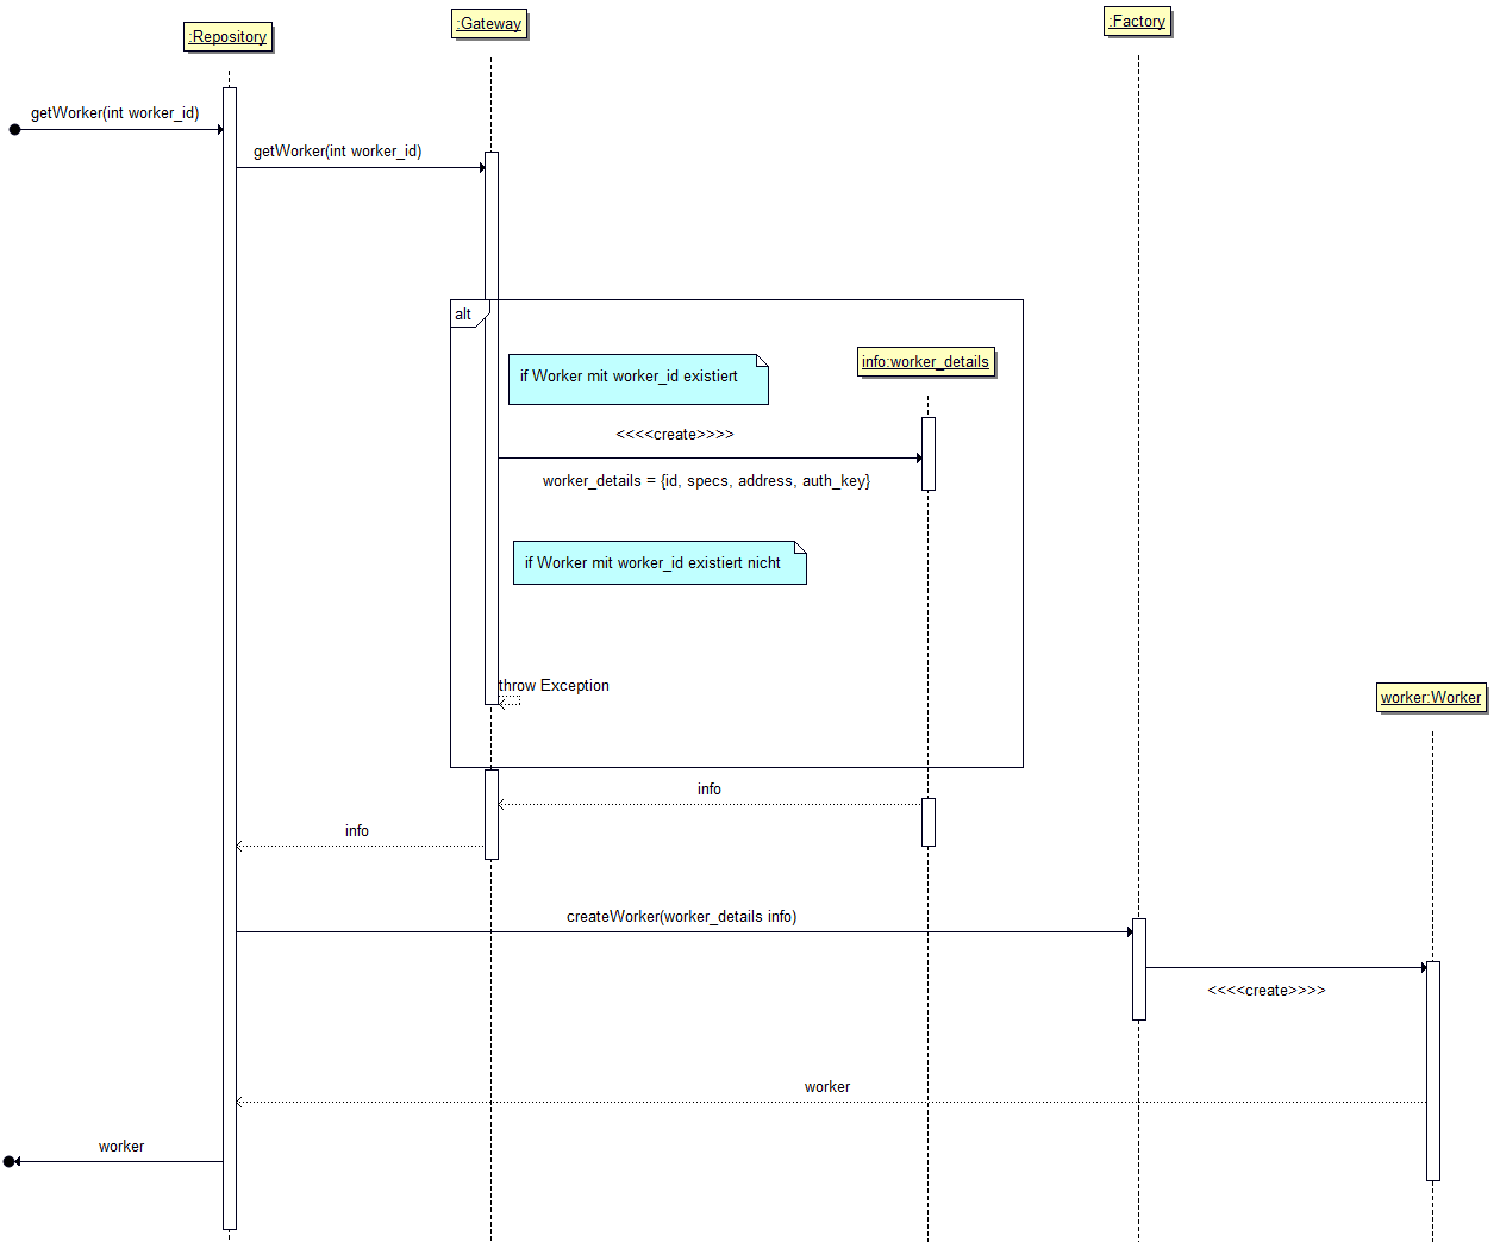
\includegraphics[width=\textwidth]{repository_sequence_diagram}

Der Rest des Programms verwendet die Repository-Klasse als Schnittstelle für Queries. \textit{public Worker getWorker(uint64\_t worker\_id)} wird aus dem Repository aufgerufen. Das Repository ruft dann die Methode \textit{getWorker} im Gateway mit dem vom Client übergebenen Argument auf. Wenn die Operation erfolgreich war, übergibt das Repository den Rückgabewert vom Gateway an die Methode \textit{createWorker} in der Factory. Das Repository gibt dann das neu erzeugte Worker-Objekt an den Client zurück.

\clearpage

\subsection{Eine neue Aufgabe einreichen}

In diesem Sequenzdiagramm ist der Ablauf einer typischen Kommunikation zwischen Client (Benutzer) und Server (Scheduler) veranschaulicht. In diesem Fall gibt der Benutzer eine neue Aufgabe in Auftrag. Andere Anfragen, wie etwa eine Statusabfrage einer vorhandenen Aufgabe finden nach einem analogen Ablauf statt.

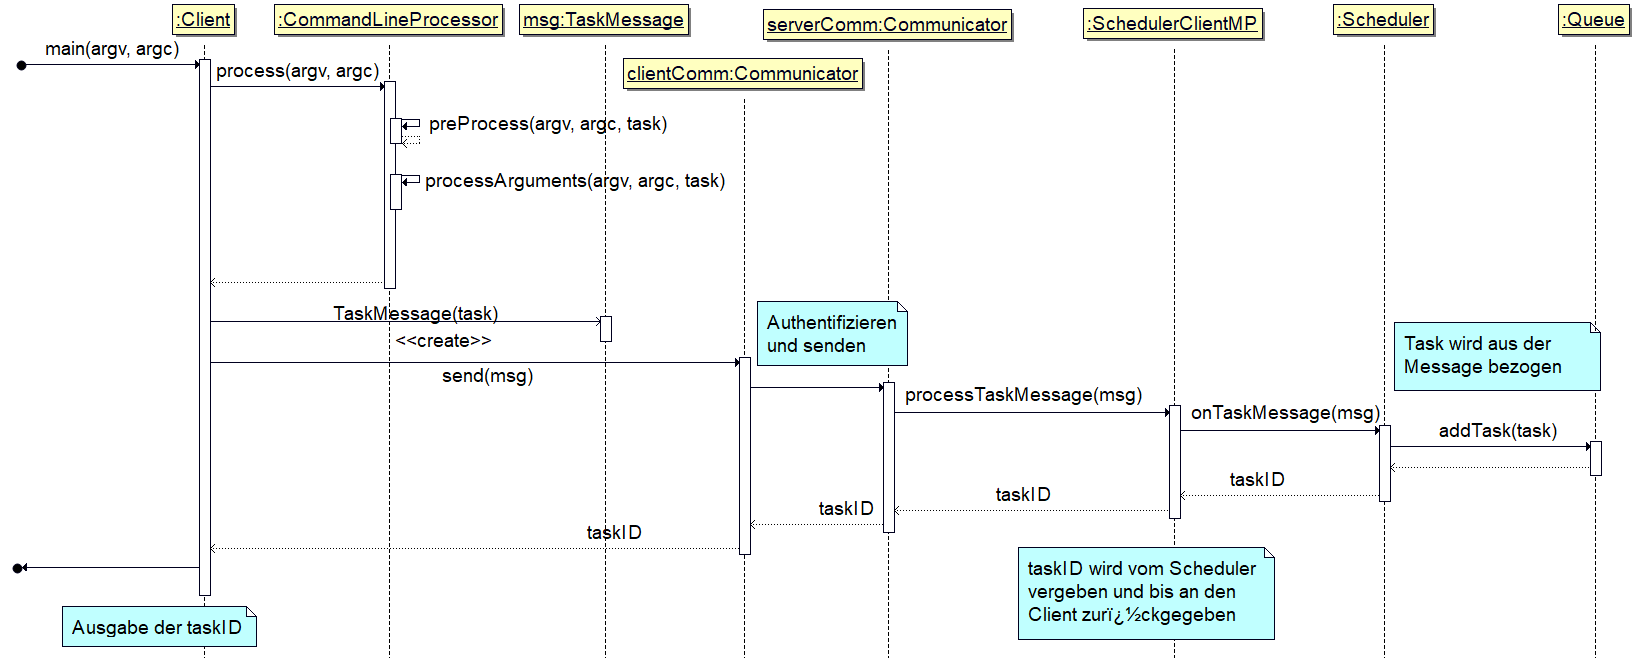
\includegraphics[width=\textwidth]{createTask}

Ein anderer Befehl des Benutzers, etwa die Nachfrage, wie der Bearbeitungsstatus einer Aufgabe derzeit ist, folgen diesem Ablauf. Sie unterscheiden sich im wesentlichen nur in den Aktionen, die auf Seiten der Server Anwendung stattfinden, sowie der Rückgabe, die der Server an den Client übermittelt.

% Document ends here.
\printnoidxglossaries

\end{document}
